
\chapter{Sprint 2}
\label{Sprint2}
\lhead{Chapter 8. \emph{Sprint 2}}

\section{Duration}
The duration of the sprint was the following:
\begin{itemize}
\item Start: September, 23rd
\item End: October, 6th
\end{itemize}

\section{Planning}

Having just demonstrated the product to the customer during the previous sprint, most of the work planned for this sprint was documentation writing in view of the second milestone.
This included writing the report itself but also reviewing other documents such as the templates, notes and agendas.

During last sprint, we agreed with the customer to prioritise interoperability with HealthVault rather than Withings.
For this purpose, we adjusted our plan accordingly and tasked one team member to study HealthVault's SDK in order to determine the complexity of the task.

Additionally, we planned to continue with development and add support for weight measurements to the API.

Although one member of the team would be working remotely from another city, we thought it would be easy for him to collaborate in writing the documentation so we did not prepare a separate work plan for him.
We did, though, schedule an internal meeting to be held weekly on Mondays to keep in touch and share information about the project's progress.


\section{Goal(s)}

The main goal for this iteration was to write the report in view of the second milestone deadline for mid-term delivery (M2). 
Additional goals were assessing the practicality of interoperability with HealthVault and adding support for weight measurements to the API.

\section{Results and feedback}

We wrote a table of contents for the report and parts of the initial chapters as well.
The table of contents was submitted to the supervisor in order to make sure we weren't leaving out any important chapter in our report. 
The team member who had moved to Oslo was able to contribute to the project by writing the report.

Studies on HealtVault went smoothly. We were confident that we could fulfill the customer requirest and came up with the idea of writing another Android application which would fetch some weight measurements from HealthVault and send them to our integration platform.
We presented this idea to the customer after a few days and he agreed on it.
We then started some preliminary development on it which proceeded smoothly.
This was also thanks to HealthVault's SDK which greatly reduced the amount of code we needed to write ourselves from scratch. 
We used one of the examples provided with the SDK which featured out-of-the-box interoperability with HealthVault and added the functionality required to implement interoperability with NIPEN.

System development also proceeded smoothly and we added support for the weight data to the backend.
The frontend and the database needed little work to accomodate these additions, so most of the work done on them were minor tweaking.

\section{Evaluation}

\begin{figure}
\centering
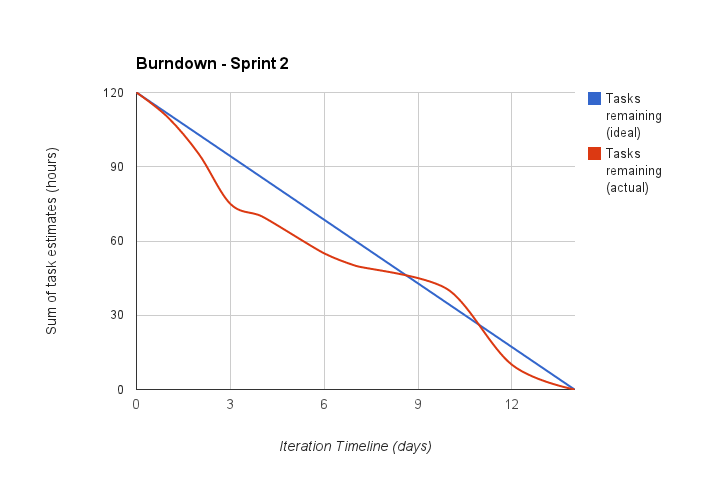
\includegraphics[scale=0.60]{../Figures/burndownSprint2.png}
\caption{Iteration burndown chart}
\label{figure:burndownsprint2}
\end{figure}

Results for this sprint were positive. We were pleased with how the report was shaping up and received good feedback on our structure from the supervisor.

Our plan to let our colleague in Oslo work on the documentation worked out pretty well and he was able to work indipendently and effeciently. 
Although he had moved to Oslo, he didn't start to work right away so he a lot of time to dedicate to the project.

Since we had told the customer that we would be working primarily on the report for this sprint, he didn't put any pressure on us to develop new features. 
We actually could not contact him the first week after the demonstration but this has not been an issue at all since we knew what to work on. 
We were happy that our project was well in schedule with our plan so far.
This iterations burndown chart is shown in figure \ref{figure:burndownsprint2}.

\clearpage
\section{Backlog}

See below the sprint backlog.
\begin{enumerate}[1.]
	\item \textbf{Project management} included:
	\begin{itemize}
		\item \textbf{Sprint startup meeting}:
			included sprint planning and review
		\item \textbf{Weekly meetings}:
			with both the customer and the supervisor
			%*During week 39.we were unable to contact the customer. This was not a problem*
		\item \textbf{Meeting notes}:
			taking notes during meetings, reviewing of the notes
		\item \textbf{Status reports}:
			for both week 39 and 40
		\item \textbf{Review templates}:
			to be adopted for status reports and other documents
		\item \textbf{Risk analysis}:
			updated on a weekly basis
	\end{itemize}
	\item \textbf{Report work}\newline
		start writing the report, focus on necessary chapters for the mid-term delivery
	\item \textbf{HealthVault studies}\newline
		perform further studies in order to assess the feasibility of developing a prototype
		application that implemented interoperability with Microsoft's platform
	\item \textbf{System development}\newline
		preliminary development on the backend to accomodate the new weight API
	\item \textbf{Weigther application development}\newline
		initial design and implementation of a prototype application using the weight API.
		The application needs to connect to HealthVault and retrieve some weight measurements
		and then send them to the integration platform.
\end{enumerate}